  \item Zmiana danych zamawiającego\\
  
  Opis słowny - niekiedy już po złożeniu zamówienia wymagana jest zmiana
  odbiorcy - albo zmiana adresu odbioru, albo osoby odpowiedzialnej czy innych
  warunków zamówienia. Sam klient nie ma uprawnień by to zrobić, ale po
  kontakcie z pracownikiem większość zmian jest możliwa.
  
  \begin{longtable}{|p{5cm}|p{7cm}|}
 	\hline
	\textbf{Aktor} & Pracownik \\
	\hline
	\textbf{Warunki początkowe} & Pracownik zalogowany, zmiany wprowadzane na
	wniosek klienta
	\\
	\hline
	\textbf{Opis przebiegu interakcji} & Wybór zarządzania zamówieniami,
	z listy zamówień zaznaczenie konkretnego, wyświetlenie okna edycji
	\\
	\hline
	\textbf{Sytuacje wyjątkowe} & Z punktu widzenia systemu brak (choć dane
	odbiorcy mogą być w rzeczywistości nieprawdziwe)
	\\
	\hline
	\textbf{Warunki końcowe} & Zmiana odbiorcy odpowiedzialnego za zamówienie
	(zapis w bazie sklepu)
	\\
	\hline
 \end{longtable}
  
  \begin{tabularx}{\linewidth}{c X}
  Aktor: & Pracownik \\
  Opis: & Można zmienić dane odbiorcy na potrzeby danego zamówienia (zmiana
  danych tylko w ramach konkretnej faktury). Dotyczy to w szczególności adresu i
  danych osobowych osoby odpowiedzialnej za zamówienie.
  \end{tabularx}  
	\begin{enumerate}
	  \item Pracownik po autoryzacji w panelu sterowania systemu, przechodzi do
	  panelu Zarządzania Zamówieniami (patrz Zamówienia przypadek użycia 1)
	  \item Z wyświetlonej przez system listy zamówień, pracownik wybiera jeden
	  element i wybiera opcję Zmień Dane Odbiorcy
	  \item System prezentuje aktualnie dane odbiorcy (mogą to być aktualne dane
	  klienta, albo już wcześniej modyfikowane dane osobowe wprowadzone specjalnie w
	  ramach tego zamówienia)
	  \item Pracownik modyfikuje wybraną przez siebie składową danych (wszystkie
	  elementy pozwalają na edycję) i zatwierdza wprowadzone zmiany
	  \item System wyświetla zapytanie o potwierdzenie zmian i po jego akceptacji
	  wysyła powiadomienie do klienta o zaszłych zmianach – wiadomość drogą
	  elektroniczną
	\end{enumerate}


\begin{figure}[H]
    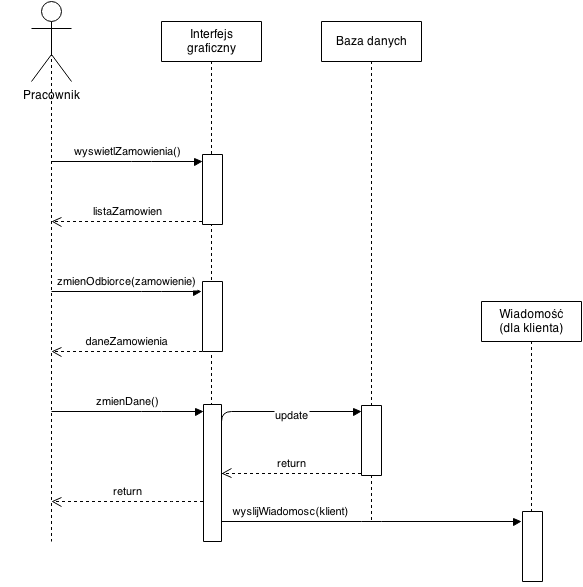
\includegraphics[width=\textwidth,
    height=0.5\textheight]{graphics/UseCase/Zamowienia/ZmianaDanychZamawiajacegoSD.png}
    \caption{Diagram sekwencji dla przypadku użycia Zmiana danych zamawiającego
    - scenariusz główny}
\end{figure}
